\section{Potenziali con orbite chiuse e limitate}\linkdest{sec:orbitso}
\begin{frame}{Potenziali centrali con orbite limitate}
\begin{block}{Teorema di Bertrand}
among central force potentials with bound orbits, there are only two types of central force potentials where all bound orbits are also closed:
\begin{itemize}
\item Inverse square central force : $V(\vec{r})=\frac{-k}{r}$
\item harmonic oscillator: $V(\vec{r})=\frac{1}{2}kr^2$
\end{itemize}
\end{block}
\end{frame}

\begin{wordonframe}{potenziale che ammette orbite chiuse}
Punto stazionario di V ( cio\'e del potenziale efficacie).
Stabilit\'a orbita: $\TtwoDy{r}{V}<0$
\url{https://arxiv.org/pdf/1411.7057.pdf}
\end{wordonframe}

\section{Orbite Kepleriane}\linkdest{sec:orbitsk}

\begin{frame}{Problema ridotto}
\begin{columns}
\begin{column}{0.3\textwidth}
\input{reducedproblem}
\begin{align*}
&m_1\ddvec{r}_1=\frac{m_1m_2G}{r^3}\vec{r}\\
&m_2\ddvec{r}_2=\frac{m_1m_2G}{r^3}\vec{r}\\
&\mu\ddvec{r}=-k^2\frac{\vec{r}}{r^3}=-\frac{\gamma}{\mu}\frac{\vec{r}}{r^3}
\end{align*}
\end{column}
\begin{column}{0.7\textwidth}
\begin{block}{Costanti del moto}
\begin{align*}
&E_T=\frac{1}{2}m_1\dvec{r}_1^2+\frac{1}{2}m_2\dvec{r}_2^2-G\frac{m_1m_2}{r}\\
&=E_{CM}+E=\frac{1}{2}m\dvec{R}^2+\frac{1}{2}\mu\dvec{r}^2-G\frac{m\mu}{r}
\end{align*}
\begin{block}{Momento angolare}
\[\vec{J}=\mu\vec{r}\wedge\dvec{r}\ \vec{J}\cdot\vec{r}=0\ \vec{J}\cdot\dvec{r}=0\]
\end{block}
\begin{block}{Vettore di Lenz}
\begin{align*}
&\vec{L}=\dvec{r}\wedge\vec{J}-\gamma\frac{\vec{r}}{r}=\dvec{r}\wedge\vec{J}-Gm_1m_2\frac{\vec{r}}{r}\\
&\dvec{L}=0\ \scap{J}{L}=0\ \scap{L}{r}=\frac{1}{\mu}J^2-\gamma r\\
&L^2=\gamma^2+\frac{2}{\mu}EJ^2
\end{align*}
\end{block}
\end{block}
\end{column}
\end{columns}
\end{frame}

\begin{wordonframe}{Definizione problema 2 corpi attrazione newtoniana}
\begin{align*}
&\vec{R}=\frac{m_1\vec{r}_1+m_2\vec{r}_2}{M}\\
&\vec{r}=\vec{r}_1-\vec{r}_2
\end{align*}
$\vec{r}$ ruota in piano perpendicolare a $\vec{J}$ e $\vec{L}$ \'e sul piano dell'orbita.

\begin{align*}
&\dvec{L}=-\nabla U\wedge(\vecp{x}{p})+\vec{p}\wedge\TDy{t}{\vec{J}}-\frac{Gm}{r}\vec{p}+ \frac{Gm^2(\scap{p}{x})}{r^3}\vec{x}\\
&=\frac{1}{r}(\TDy{r}{U}-\frac{k}{r^2})(r^2\vec{p}-(\scap{x}{p})\vec{x})\\
&k=mG,\ \nabla U=-\mu\ddvec{r}=\TDy{r}{U}\frac{\vec{x}}{r} 
\end{align*}

\end{wordonframe}

\begin{frame}{forma dell'orbita}
\begin{columns}
\begin{column}{0.4\textwidth}
\input{conservedvector}
\begin{block}{Periodo orbitale}
\begin{align*}
&JT=2\mu\pi ab\\
&T=2\pi\sqrt{\frac{a^3}{k^2}}\\
&n^2a^3=Gm(=m_1+m_2)
\end{align*}
\end{block}
\end{column}
\begin{column}{0.6\textwidth}
\begin{align*}
&Lr\cos{v}+\gamma r=\frac{1}{\mu}J^2\\
&r=\frac{p}{1+e\cos{v}}\\
&p=\frac{J^2}{\gamma\mu},\ e=\frac{L}{\gamma}
\end{align*}
\begin{block}{Orbite ellittiche: $E<0,\ e<1$.}
\begin{align*}
&r_{min}=\frac{p}{1+e},\ r_{max}=\frac{p}{1-e}\\
&a=\frac{1}{2}(r_{min}+r_{max})=\frac{p}{1-e^2}\\
&=\frac{h^2}{Gm(1-e^2)}=-\frac{\gamma}{2E}\\
&J_{max}=\gamma\sqrt{\frac{\mu}{2|E|}}
\end{align*}
\end{block}
\end{column}
\end{columns}
\end{frame}

\begin{wordonframe}{Orbita kepleriana}
\begin{columns}[T]
\begin{column}{0.45\textwidth}
L'orbita \'e una conica con asse lungo $\vec{L}$, il modulo di L dipende da E e J:
\begin{align*}
&e\gtreqless1\Leftrightarrow L\gtreqless\gamma\Leftrightarrow E\gtreqless0\\
&a=\frac{\gamma}{2|E|}\\
&b/a=\sqrt{1-e^2}
\end{align*}
connessione tra aspetti geometrici e dinamici: $a=-\frac{\gamma}{2E}$.
\end{column}
\begin{column}{0.55\textwidth}
\begin{block}{Velocit\'a}
\begin{align*}
&v^2=Gm(\frac{2}{r}-\frac{1}{a})\\
&\dot{r}=\frac{h^2e\sin{f}}{Gm(1+e\cos{f})^2}\TDy{t}{f}=\frac{Gm}{h}e\sin{f}\\
&r\dot{\theta}=\frac{h}{r}=\frac{Gm}{h}(1+e\cos{f})
\end{align*}
\end{block}
\end{column}
\end{columns}
Per una certa energia E J non pu\'o superare quel valore per cui $a=b$.
\begin{align*}
&dS=\frac{1}{2}rr\dot{\theta}\,dt\\
&J=2\mu\TDy{t}{S}
\end{align*}
Terza legge di Keplero: $T\propto a\expy{\frac{3}{2}}$ (per pianeti maggiori sistema solare $\msun{}/m\approx\num{e-3}$).
moto medio $\frac{2\pi}{T}$: $n^2a^3=k^2$.
\end{wordonframe}

\begin{wordonframe}{Terza legge di Keplero}
\begin{columns}[c]\begin{column}{0.7\textwidth}
\begin{align*}
&\ddvec{r}_1-\ddvec{r}_2=-\frac{G(m_1+m_2)}{|\vec{r}_1-\vec{r}_2|^3}(\vec{r}_1-\vec{r}_2)
\end{align*}
\end{column} \begin{column}{0.3\textwidth}
\begin{align*}
&P^2=\frac{4\pi^2}{G(m_1+m_2)}a^3
\end{align*}
\end{column}  \end{columns}
\begin{columns}[c]\begin{column}{0.7\textwidth}
\begin{align*}
&m_1\vec{r}_1+m_2\vec{r}_2=0\\
&\vec{r}_1-\vec{r}_2=\frac{m_1+m_2}{m_2}\vec{r}_1=-\frac{m_2+m_1}{m_1}\vec{r}_2\\
&m_1\ddvec{r}_1=-Gm_1m_2\frac{m_2^3}{(m_1+m_2)^3r_1^3}\frac{m_1+m_2}{m_2}\vec{r}_1\\
&\ddvec{r}_1=-\frac{\mu_1}{r_1^3}\vec{r}_1\\
&\ddvec{r}_2=-\frac{\mu_2}{r_2^3}\vec{r}_2
\end{align*}
\end{column} \begin{column}{0.3\textwidth}
\begin{align*}
&P^2=\frac{4\pi^2}{\mu_1}a_1^3\\
&P^2=\frac{4\pi^2}{\mu_2}a_2^3
\end{align*}
\end{column}  \end{columns}
\end{wordonframe}

\begin{frame}{Elementi orbitali}
%\documentclass[border=5pt]{standalone}
%\usepackage{tikz,tikz-3dplot}

\tdplotsetmaincoords{70}{110}
\begin{tikzpicture}[tdplot_main_coords,scale=5]
  \pgfmathsetmacro{\r}{.8}
  \pgfmathsetmacro{\O}{45} % right ascension of ascending node [deg]
  \pgfmathsetmacro{\i}{30} % inclination [deg]
  \pgfmathsetmacro{\f}{35} % true anomaly [deg]

  \coordinate (O) at (0,0,0);

  \draw [->] (O) -- (1.7,0,0) node[anchor=north east] {$x$};
  \draw [->] (O) -- (0,1,0) node[anchor=north west] {$y$};
  \draw [->] (O) -- (0,0,1) node[anchor=south] {$z$};

  \node at (0,-\r,0) [left,text width=4em] {Ecliptic Plane};

  \tdplotdrawarc[dashed]{(O)}{\r}{0}{360}{}{}

  \tdplotsetrotatedcoords{\O}{0}{0}

  \draw [tdplot_rotated_coords] (-1,0,0) -- (1,0,0) node [below right] {Line of Nodes};
  \tdplotdrawarc[->]{(O)}{.33*\r}{0}{\O}{anchor=north}{$\Omega$}

  \tdplotsetrotatedcoords{-\O}{\i}{0}
  \tdplotdrawarc[tdplot_rotated_coords]{(O)}{\r}{0}{360}{}{}  
  \begin{scope}[tdplot_rotated_coords]
    % \draw[->] (O) -- (1,0,0) node [above] {$x'$};
    % \draw[->] (O) -- (0,1,0) node [above] {$y'$};
    \draw[->] (O) -- (0,0,1) node [above] {$\hat{h}$};
    \draw (1,0,0) -- (-1,0,0) node[above] {Semi-major axis};
     \tdplotdrawarc[->]{(O)}{.33*\r}{90}{180}{anchor=west}{$\omega$}
    \coordinate (P) at (180+\f:\r);
    \draw (O) -- (P);
    \tdplotdrawarc[->]{(O)}{.33*\r}{180}{180+\f}{anchor=south west}{$\nu$}
  \end{scope}

  \tdplotsetrotatedcoords{-\O+\f}{\i}{0}
  \tdplotsetrotatedcoordsorigin{(P)}
  \begin{scope}[tdplot_rotated_coords,scale=.2,thick]
    \draw [->] (P) -- (-1,0,0) node [right] {$\hat{r}$};
    \draw [->] (P) -- (0,-1,0) node [above] {$\hat{\theta}$};
    \draw [->] (P) -- (0,0,1) node [above] {$\hat{k}$};
    \fill (P) circle (.33ex);
  \end{scope}

  \tdplotsetthetaplanecoords{-\f}
  \tdplotdrawarc[tdplot_rotated_coords,->]{(O)}{.75*\r}{0}{\i}{anchor=south}{$i$} % not accurate :(
\end{tikzpicture}

\end{frame}

\begin{wordonframe}{Elementi orbitali}
Piano ecclittica: piano orbita solare rif geocentrico: ''intersezione della sfera celeste con il piano su cui giace l'orbita terrestre
Linea dei nodi \'e intersezione tra piano orbita pianeta e piano eclittica, i \'e l'inclinazione del piano dell'orbita rispetto al piano dell'eclittica.
L'angolo $\Omega$ identifica l'orientazione della linea dei nodi rispetto al punto $\gamma$ posizione del Sole all'equinozio di primavera; l'angolo $\omega$ identifica la direzione del semi-asse maggiore rispetto alla linea dei nodi; l'angolo $\nu$ identifica la posizione del pianeta sull'orbita.
\end{wordonframe}

\begin{frame}{Orbite Kepleriane - legge del moto.}
\begin{columns}
\begin{column}{0.2\textwidth}
\begin{figure}[!ht]
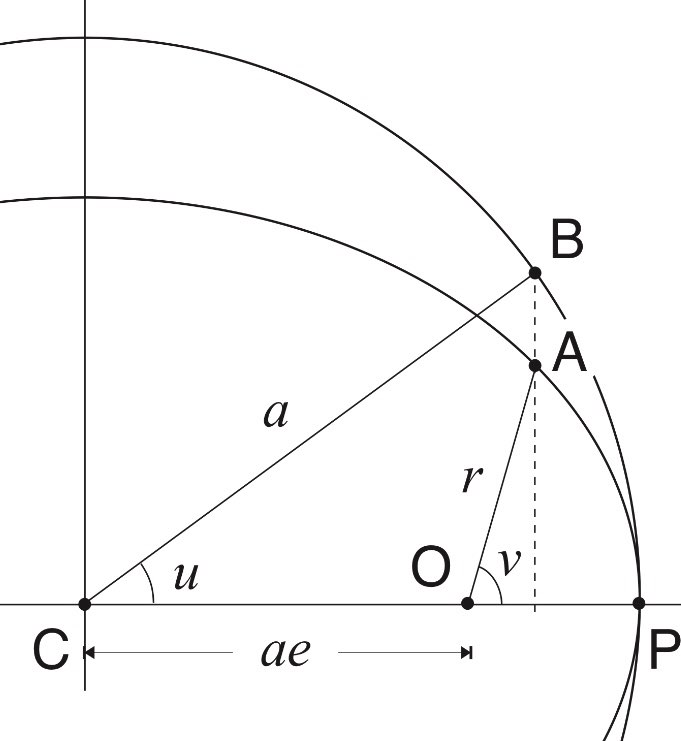
\includegraphics[width=\textwidth]{ellipseinO}
\end{figure}
\end{column}
\begin{column}{0.8\textwidth}
\begin{block}{Anomalia eccentrica}
\begin{align*}
&r\cos{\nu}=a\cos{u}-ae\\
&\pi\frac{ab}{T}=\frac{1}{2}nab=\frac{1}{2}r^2\dot{v}=\frac{1}{2}br\dot{u}\\
&=\frac{1}{2}ab(1-e\cos{u})\dot{u}=\frac{1}{2}ab\TDof{t}(u-e\sin{u})
\end{align*}
\end{block}
\end{column}
\end{columns}
\begin{block}{Anomalia media: equazione di Keplero}
\begin{align*}\label{eq:Keq}
&\phi=u-e\sin{u}\Rightarrow\dot{\phi}=n
\end{align*}
\end{block}
\end{frame}

\begin{wordonframe}{legge oraria}
u \'e detta anomalia eccentrica
Relazioni trigonometriche tra ue $\nu$
\begin{align*}
&a(1-e\cos{u})=\frac{p}{1+\cos{\nu}}\\
&\tg{\nu/2}=\sqrt{\frac{1+e}{1-e}}\tg{u/2}
\end{align*}
$\phi(t)=\phi_0+nt=n(t-t_0)$: $\phi_0$ \'e l'istante in cui $\phi=\nu=0$.
Il problema \'e caratterizzato da 6 costanti: $E$, $J_x$, $J_y$, $J_z$, $\nu$ (direzione di $\vec{L}$), $t_0$.
L'equazione di Keplero \refeq{eq:Keq}, noti n e $t_0$, fornisce $\phi(t)$ e quindi $u(t)$ e ancora $r(t)$ e $\nu(t)$.
\end{wordonframe}

\begin{frame}{Approx. piccola eccentricit\'a}
\begin{figure}[!ht]
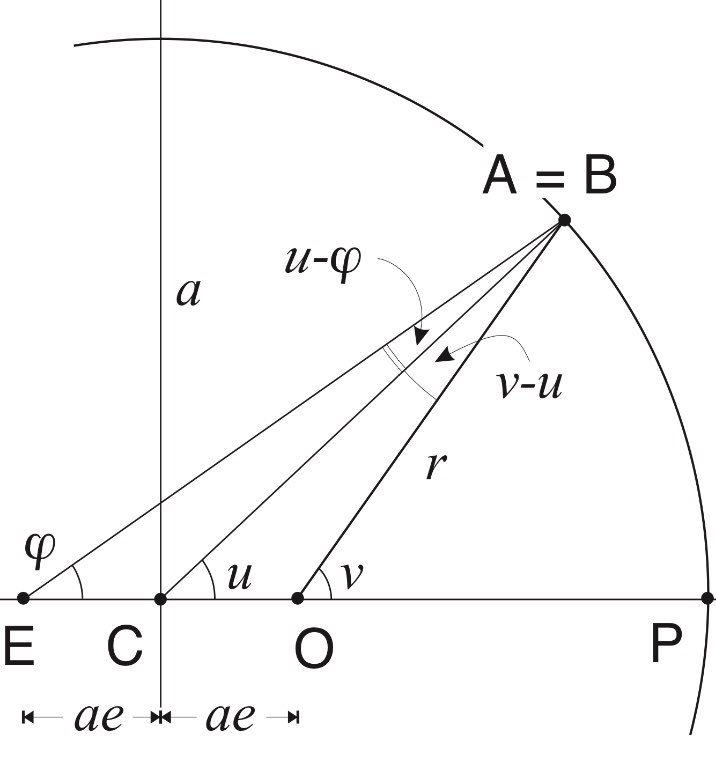
\includegraphics[width=0.5\textwidth]{tolomeo}
\end{figure}
\end{frame}

\begin{wordonframe}{orbita quasi circolare}
$\sqrt{\frac{1+e}{1-e}}\approx1+e$
$v\approx\phi+2e\sin{\phi}$
equante di Tolomeo: l'angolo in E \'e $\phi$ a meno di $e^2$
\end{wordonframe}
